% Options for packages loaded elsewhere
\PassOptionsToPackage{unicode}{hyperref}
\PassOptionsToPackage{hyphens}{url}
%
\documentclass[
  12pt,
]{article}
\title{Comparison of Physical Characteristics, Avian Clutch Size, and
Mating Tactics}
\usepackage{etoolbox}
\makeatletter
\providecommand{\subtitle}[1]{% add subtitle to \maketitle
  \apptocmd{\@title}{\par {\large #1 \par}}{}{}
}
\makeatother
\subtitle{\url{https://github.com/jcf55/Fahrenholz_Costes_ENV872_EDA_FinalProject}}
\author{Lydie Costes and Jackie Fahrenholz}
\date{}

\usepackage{amsmath,amssymb}
\usepackage{lmodern}
\usepackage{iftex}
\ifPDFTeX
  \usepackage[T1]{fontenc}
  \usepackage[utf8]{inputenc}
  \usepackage{textcomp} % provide euro and other symbols
\else % if luatex or xetex
  \usepackage{unicode-math}
  \defaultfontfeatures{Scale=MatchLowercase}
  \defaultfontfeatures[\rmfamily]{Ligatures=TeX,Scale=1}
  \setmainfont[]{Times New Roman}
\fi
% Use upquote if available, for straight quotes in verbatim environments
\IfFileExists{upquote.sty}{\usepackage{upquote}}{}
\IfFileExists{microtype.sty}{% use microtype if available
  \usepackage[]{microtype}
  \UseMicrotypeSet[protrusion]{basicmath} % disable protrusion for tt fonts
}{}
\makeatletter
\@ifundefined{KOMAClassName}{% if non-KOMA class
  \IfFileExists{parskip.sty}{%
    \usepackage{parskip}
  }{% else
    \setlength{\parindent}{0pt}
    \setlength{\parskip}{6pt plus 2pt minus 1pt}}
}{% if KOMA class
  \KOMAoptions{parskip=half}}
\makeatother
\usepackage{xcolor}
\IfFileExists{xurl.sty}{\usepackage{xurl}}{} % add URL line breaks if available
\IfFileExists{bookmark.sty}{\usepackage{bookmark}}{\usepackage{hyperref}}
\hypersetup{
  pdftitle={Comparison of Physical Characteristics, Avian Clutch Size, and Mating Tactics},
  pdfauthor={Lydie Costes and Jackie Fahrenholz},
  hidelinks,
  pdfcreator={LaTeX via pandoc}}
\urlstyle{same} % disable monospaced font for URLs
\usepackage[margin=2.54cm]{geometry}
\usepackage{color}
\usepackage{fancyvrb}
\newcommand{\VerbBar}{|}
\newcommand{\VERB}{\Verb[commandchars=\\\{\}]}
\DefineVerbatimEnvironment{Highlighting}{Verbatim}{commandchars=\\\{\}}
% Add ',fontsize=\small' for more characters per line
\usepackage{framed}
\definecolor{shadecolor}{RGB}{248,248,248}
\newenvironment{Shaded}{\begin{snugshade}}{\end{snugshade}}
\newcommand{\AlertTok}[1]{\textcolor[rgb]{0.94,0.16,0.16}{#1}}
\newcommand{\AnnotationTok}[1]{\textcolor[rgb]{0.56,0.35,0.01}{\textbf{\textit{#1}}}}
\newcommand{\AttributeTok}[1]{\textcolor[rgb]{0.77,0.63,0.00}{#1}}
\newcommand{\BaseNTok}[1]{\textcolor[rgb]{0.00,0.00,0.81}{#1}}
\newcommand{\BuiltInTok}[1]{#1}
\newcommand{\CharTok}[1]{\textcolor[rgb]{0.31,0.60,0.02}{#1}}
\newcommand{\CommentTok}[1]{\textcolor[rgb]{0.56,0.35,0.01}{\textit{#1}}}
\newcommand{\CommentVarTok}[1]{\textcolor[rgb]{0.56,0.35,0.01}{\textbf{\textit{#1}}}}
\newcommand{\ConstantTok}[1]{\textcolor[rgb]{0.00,0.00,0.00}{#1}}
\newcommand{\ControlFlowTok}[1]{\textcolor[rgb]{0.13,0.29,0.53}{\textbf{#1}}}
\newcommand{\DataTypeTok}[1]{\textcolor[rgb]{0.13,0.29,0.53}{#1}}
\newcommand{\DecValTok}[1]{\textcolor[rgb]{0.00,0.00,0.81}{#1}}
\newcommand{\DocumentationTok}[1]{\textcolor[rgb]{0.56,0.35,0.01}{\textbf{\textit{#1}}}}
\newcommand{\ErrorTok}[1]{\textcolor[rgb]{0.64,0.00,0.00}{\textbf{#1}}}
\newcommand{\ExtensionTok}[1]{#1}
\newcommand{\FloatTok}[1]{\textcolor[rgb]{0.00,0.00,0.81}{#1}}
\newcommand{\FunctionTok}[1]{\textcolor[rgb]{0.00,0.00,0.00}{#1}}
\newcommand{\ImportTok}[1]{#1}
\newcommand{\InformationTok}[1]{\textcolor[rgb]{0.56,0.35,0.01}{\textbf{\textit{#1}}}}
\newcommand{\KeywordTok}[1]{\textcolor[rgb]{0.13,0.29,0.53}{\textbf{#1}}}
\newcommand{\NormalTok}[1]{#1}
\newcommand{\OperatorTok}[1]{\textcolor[rgb]{0.81,0.36,0.00}{\textbf{#1}}}
\newcommand{\OtherTok}[1]{\textcolor[rgb]{0.56,0.35,0.01}{#1}}
\newcommand{\PreprocessorTok}[1]{\textcolor[rgb]{0.56,0.35,0.01}{\textit{#1}}}
\newcommand{\RegionMarkerTok}[1]{#1}
\newcommand{\SpecialCharTok}[1]{\textcolor[rgb]{0.00,0.00,0.00}{#1}}
\newcommand{\SpecialStringTok}[1]{\textcolor[rgb]{0.31,0.60,0.02}{#1}}
\newcommand{\StringTok}[1]{\textcolor[rgb]{0.31,0.60,0.02}{#1}}
\newcommand{\VariableTok}[1]{\textcolor[rgb]{0.00,0.00,0.00}{#1}}
\newcommand{\VerbatimStringTok}[1]{\textcolor[rgb]{0.31,0.60,0.02}{#1}}
\newcommand{\WarningTok}[1]{\textcolor[rgb]{0.56,0.35,0.01}{\textbf{\textit{#1}}}}
\usepackage{longtable,booktabs,array}
\usepackage{calc} % for calculating minipage widths
% Correct order of tables after \paragraph or \subparagraph
\usepackage{etoolbox}
\makeatletter
\patchcmd\longtable{\par}{\if@noskipsec\mbox{}\fi\par}{}{}
\makeatother
% Allow footnotes in longtable head/foot
\IfFileExists{footnotehyper.sty}{\usepackage{footnotehyper}}{\usepackage{footnote}}
\makesavenoteenv{longtable}
\usepackage{graphicx}
\makeatletter
\def\maxwidth{\ifdim\Gin@nat@width>\linewidth\linewidth\else\Gin@nat@width\fi}
\def\maxheight{\ifdim\Gin@nat@height>\textheight\textheight\else\Gin@nat@height\fi}
\makeatother
% Scale images if necessary, so that they will not overflow the page
% margins by default, and it is still possible to overwrite the defaults
% using explicit options in \includegraphics[width, height, ...]{}
\setkeys{Gin}{width=\maxwidth,height=\maxheight,keepaspectratio}
% Set default figure placement to htbp
\makeatletter
\def\fps@figure{htbp}
\makeatother
\setlength{\emergencystretch}{3em} % prevent overfull lines
\providecommand{\tightlist}{%
  \setlength{\itemsep}{0pt}\setlength{\parskip}{0pt}}
\setcounter{secnumdepth}{5}
\ifLuaTeX
  \usepackage{selnolig}  % disable illegal ligatures
\fi

\begin{document}
\maketitle

\newpage
\tableofcontents 
\newpage
\listoftables 
\listoffigures 
\newpage

\hypertarget{rationale-and-research-questions}{%
\section{Rationale and Research
Questions}\label{rationale-and-research-questions}}

According to the study from which this data was extracted, avian body
size and the evolution of birds over time is a subject matter that has
generated much debate. Generally, there is agreement around the idea
that body size of bird species relates to other characteristics, but the
role of evolution continues to be disputed. This project intends to
explore the correlation between tail length and other characteristics in
our data.

First, we ask the question if female tail length predicts clutch size.
Tail length has a significant impact on control and agility (Evans
1999). Longer tails increase crash risk as well as reduce the ability to
maneuver (Evans 1999). We believe that tail length may have an overall
negative impact on clutch size, as birds with longer tail lengths may be
less efficient at collecting food for their young.

Second, we will explore interactions between male tail length and
methods of display, mating system, and resource sharing systems. As
stated above, tail length likely has a negative impact on navigation and
collecting food, but male tail length has a positive impact on sexual
display for many species. Physical characteristics of males are
evaluated by females in search of a mate, but the importance of tail
length may vary greatly by species.

\begin{figure}
\centering
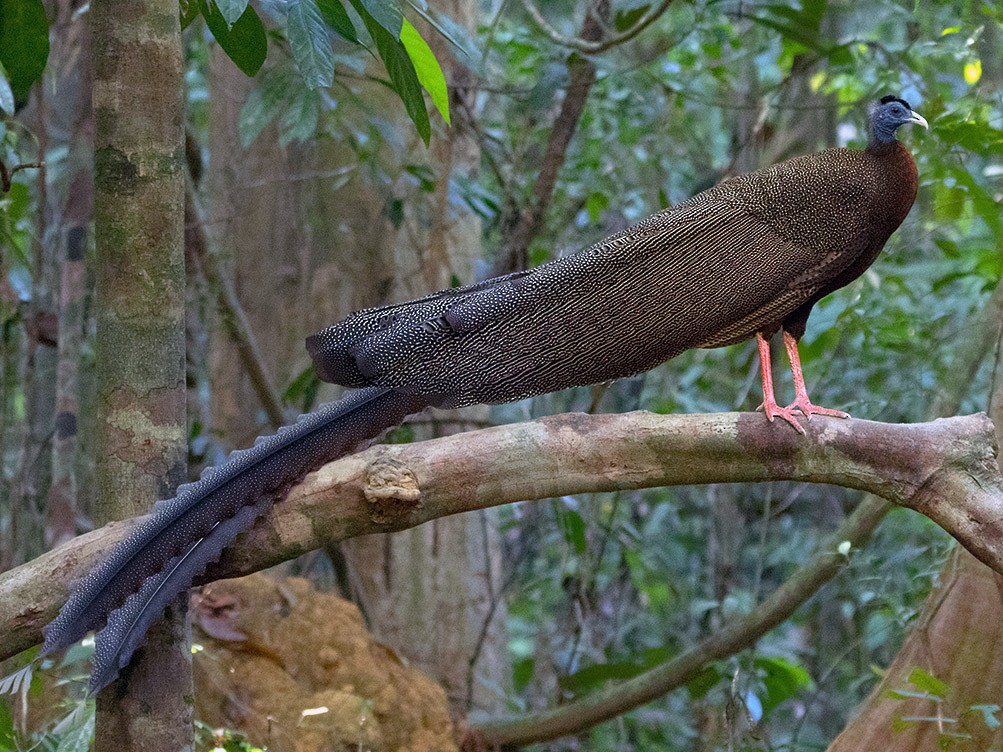
\includegraphics{Images/crested_argus_pheasant.jpeg}
\caption{A male Great Argus (\emph{Argusianus argus})}
\end{figure}

\hypertarget{dataset-information}{%
\section{Dataset Information}\label{dataset-information}}

Our dataset consists of ornithological data that was collected starting
in 2005 and was last updated in January of 2007. Data for this
collection come from regions that include:

\begin{itemize}
\tightlist
\item
  Western Palearctic
\item
  Neararctic
\item
  Africa
\item
  Australia
\item
  New Zealand
\item
  Antarctica
\end{itemize}

The complete dataset (represented by the object \textbf{\texttt{birds}})
includes 41 variables and represents 125 families. According to the
metadata, the majority of this information was gathered from
ornithological handbooks, with some data obtained from personal
communications with authors who published information on species bird
groups. More information on the sources used can be found at:
\url{https://esapubs.org/archive/ecol/E088/096/metadata.htm} (also in
/Data/Raw in the .tex file)

\newpage

\hypertarget{exploration-of-raw-data}{%
\section{Exploration of Raw Data}\label{exploration-of-raw-data}}

View dimensions, column names, variable type, and head of each column:

\begin{verbatim}
## 'data.frame':    3769 obs. of  41 variables:
##  $ Family          : int  115 101 116 116 116 116 116 116 116 116 ...
##  $ Species_number  : int  5351 3964 5402 5398 5400 5401 5396 5405 5404 5397 ...
##  $ Species_name    : chr  "Acanthagenys rufogularis" "Acanthisitta chloris" "Acanthiza chrysorrhoa" "Acanthiza ewingii" ...
##  $ English_name    : chr  "Spiny-cheeked Honeyeater" "Rifleman" "Yellow-rumped Thornbill" "Tasmanian Thornbill" ...
##  $ Subspecies      : chr  "-999" "-999" "leighi" "ewingii" ...
##  $ M_mass          : num  47.1 5.6 9.4 7.2 7.2 5.8 6.8 7.6 6.5 7.4 ...
##  $ M_mass_N        : int  4 33 25 16 43 16 10 25 27 37 ...
##  $ F_mass          : num  41.4 7 9.8 6.7 6.9 5.7 6.7 7.4 6.3 6.5 ...
##  $ F_mass_N        : int  5 20 16 19 76 12 7 27 23 20 ...
##  $ unsexed_mass    : num  -999 -999 -999 -999 -999 -999 -999 -999 -999 -999 ...
##  $ unsexed_mass_N  : int  -999 -999 -999 -999 -999 -999 -999 -999 -999 -999 ...
##  $ M_wing          : num  113.1 47.8 57.8 52.7 48.9 ...
##  $ M_wing_N        : int  25 10 25 21 28 29 11 36 25 52 ...
##  $ F_wing          : num  107.5 51.4 57.6 51 47 ...
##  $ F_wing_N        : num  21 10 26 22 26 25 7 26 29 30 ...
##  $ Unsexed_wing    : num  -999 -999 -999 -999 -999 -999 -999 -999 -999 -999 ...
##  $ Unsexed_wing_N  : int  -999 -999 -999 -999 -999 -999 -999 -999 -999 -999 ...
##  $ M_tarsus        : num  26.2 19.1 17.7 21.3 18 18.4 18.5 17.5 17.4 20.3 ...
##  $ M_tarsus_N      : int  10 10 23 21 28 29 11 36 25 51 ...
##  $ F_tarsus        : num  25.7 19.7 17.4 21.7 17.8 17.6 18.4 17.5 17.3 19.3 ...
##  $ F_tarsus_N      : int  5 7 24 23 25 25 7 25 27 29 ...
##  $ Unsexed_tarsus  : num  -999 -999 -999 -999 -999 -999 -999 -999 -999 -999 ...
##  $ Unsexed_tarsus_N: int  -999 -999 -999 -999 -999 -999 -999 -999 -999 -999 ...
##  $ M_bill          : num  26.8 13.2 11.9 11 11.3 9.7 11.6 10.2 10 11 ...
##  $ M_bill_N        : int  8 6 24 21 27 28 11 26 24 51 ...
##  $ F_bill          : num  25.5 14.4 11.7 10.9 11.4 9.6 11.2 9.9 10 10.5 ...
##  $ F_bill_N        : num  10 7 26 23 25 24 7 26 28 29 ...
##  $ Unsexed_bill    : num  -999 -999 -999 -999 -999 -999 -999 -999 -999 -999 ...
##  $ Unsexed_bill_N  : int  -999 -999 -999 -999 -999 -999 -999 -999 -999 -999 ...
##  $ M_tail          : num  113.4 23.3 40.8 47.8 36.3 ...
##  $ M_tail_N        : int  25 10 28 21 34 28 11 36 14 51 ...
##  $ F_tail          : num  106.4 22.1 39.3 46.8 35.4 ...
##  $ F_tail_N        : int  21 7 26 23 55 25 6 26 10 30 ...
##  $ Unsexed_tail    : num  -999 -999 -999 -999 -999 -999 -999 -999 -999 -999 ...
##  $ Unsexed_tail_N  : int  -999 -999 -999 -999 -999 -999 -999 -999 -999 -999 ...
##  $ Clutch_size     : num  2.2 4 3.5 3.5 3 3 2.5 3 3 3 ...
##  $ Egg_mass        : num  5.45 1.34 1.44 1.46 1.35 0.93 -999 1.32 1.34 1.4 ...
##  $ Mating_System   : int  2 2 2 2 2 -999 -999 2 2 2 ...
##  $ Display         : int  3 1 1 1 -999 1 -999 2 -999 1 ...
##  $ Resource        : int  2 2 1 0 1 1 -999 0 -999 2 ...
##  $ References      : chr  "1, 21" "21" "1, 22, 31 " "22, 31" ...
\end{verbatim}

\newpage

\hypertarget{data-wrangling}{%
\section{Data Wrangling}\label{data-wrangling}}

After the raw dataset had been explored, it was wrangled to better suit
our analyses. Unavailable datapoints were recoded from ``-999'' to
``NA'', to be recognized by R as unavailable. Other variables were
re-coded as needed. A genus column was added, and the dataset was
modified to include only the following variables:

\begin{itemize}
\tightlist
\item
  Family
\item
  Genus
\item
  Species Name
\item
  Mass (both female and male)
\item
  Tail Length (both female and male)
\item
  Clutch Size
\item
  Mating System
\item
  Display System
\item
  Resource Sharing
\end{itemize}

This dataset was saved as \textbf{``birds.subset''} and used for
subsequent analyses. Finally, a second exploratory dataset was created
to summarize the variables of interest by family. If further time
allowed, the authors would have liked to group by higher taxonomic
level, but this information was not readily accessible.

\newpage

\hypertarget{exploration-of-processed-data}{%
\section{Exploration of Processed
Data}\label{exploration-of-processed-data}}

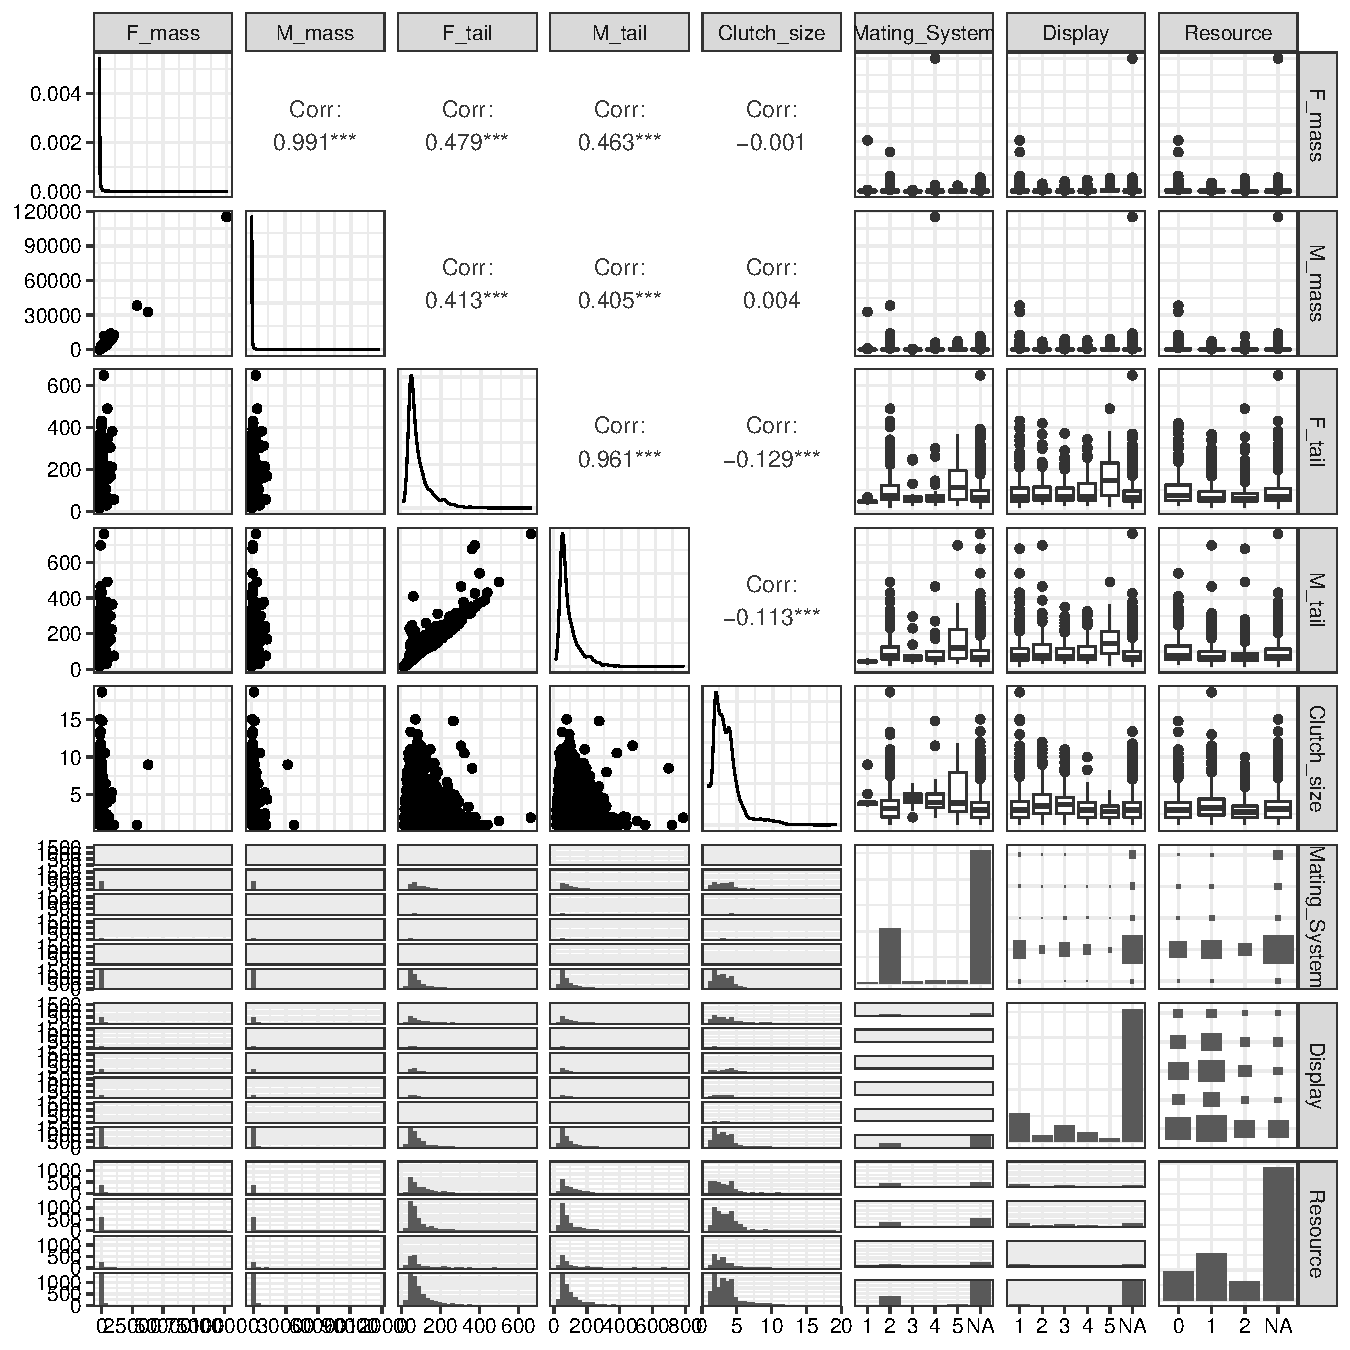
\includegraphics{Project_Code_files/figure-latex/gg exploration-1.pdf}

\newpage

\begin{longtable}[]{@{}lrrrrrrrr@{}}
\caption{Summary Statistics for Continuous Variables}\tabularnewline
\toprule
& vars & n & mean & sd & min & max & range & se \\
\midrule
\endfirsthead
\toprule
& vars & n & mean & sd & min & max & range & se \\
\midrule
\endhead
F\_mass & 1 & 2706 & 411.472616 & 2320.49997 & 1.8 & 100000.0 & 99998.2
& 44.6085053 \\
M\_mass & 2 & 2822 & 436.692275 & 2585.46747 & 2.0 & 115000.0 & 114998.0
& 48.6699134 \\
F\_tail & 3 & 2352 & 88.340901 & 59.91081 & 15.4 & 647.5 & 632.1 &
1.2353402 \\
M\_tail & 4 & 2390 & 92.410126 & 64.27592 & 15.8 & 762.0 & 746.2 &
1.3147688 \\
Clutch\_size & 5 & 2392 & 3.448037 & 1.88880 & 1.0 & 18.6 & 17.6 &
0.0386194 \\
\bottomrule
\end{longtable}

\begin{longtable}[]{@{}lrrr@{}}
\caption{Summary Statistics for Mating System}\tabularnewline
\toprule
Mating\_System & freq & pct\_valid & pct\_tot \\
\midrule
\endfirsthead
\toprule
Mating\_System & freq & pct\_valid & pct\_tot \\
\midrule
\endhead
1 & 23 & 1.888341 & 0.6102414 \\
2 & 1057 & 86.781609 & 28.0445742 \\
3 & 36 & 2.955665 & 0.9551605 \\
4 & 46 & 3.776683 & 1.2204829 \\
5 & 56 & 4.597701 & 1.4858053 \\
& 2551 & NA & 67.6837357 \\
\bottomrule
\end{longtable}

\begin{longtable}[]{@{}lrrr@{}}
\caption{Summary Statistics for Display System}\tabularnewline
\toprule
Display & freq & pct\_valid & pct\_tot \\
\midrule
\endfirsthead
\toprule
Display & freq & pct\_valid & pct\_tot \\
\midrule
\endhead
1 & 549 & 45.073892 & 14.566198 \\
2 & 118 & 9.688013 & 3.130804 \\
3 & 311 & 25.533662 & 8.251526 \\
4 & 186 & 15.270936 & 4.934996 \\
5 & 54 & 4.433497 & 1.432741 \\
& 2551 & NA & 67.683736 \\
\bottomrule
\end{longtable}

\begin{longtable}[]{@{}lrrr@{}}
\caption{Summary Statistics for Resource System}\tabularnewline
\toprule
Resource & freq & pct\_valid & pct\_tot \\
\midrule
\endfirsthead
\toprule
Resource & freq & pct\_valid & pct\_tot \\
\midrule
\endhead
0 & 480 & 30.49555 & 12.735474 \\
1 & 780 & 49.55527 & 20.695145 \\
2 & 314 & 19.94917 & 8.331122 \\
& 2195 & NA & 58.238259 \\
\bottomrule
\end{longtable}

\newpage

\hypertarget{female-versus-male-tail-length}{%
\subsubsection{Female versus Male Tail
Length}\label{female-versus-male-tail-length}}

As part of our exploration, we ran a regression to assess how correlated
male and female tail lengths are.

\begin{verbatim}
## 
## Call:
## lm(formula = M_tail ~ F_tail, data = birds.subset)
## 
## Residuals:
##    Min     1Q Median     3Q    Max 
## -46.84  -3.21  -1.27   0.85 345.40 
## 
## Coefficients:
##             Estimate Std. Error t value Pr(>|t|)    
## (Intercept) 1.226565   0.652716   1.879   0.0603 .  
## F_tail      1.033250   0.006115 168.974   <2e-16 ***
## ---
## Signif. codes:  0 '***' 0.001 '**' 0.01 '*' 0.05 '.' 0.1 ' ' 1
## 
## Residual standard error: 17.76 on 2348 degrees of freedom
##   (1419 observations deleted due to missingness)
## Multiple R-squared:  0.924,  Adjusted R-squared:  0.924 
## F-statistic: 2.855e+04 on 1 and 2348 DF,  p-value: < 2.2e-16
\end{verbatim}

The answer is yes, they are correlated (p \textless{} 0.001, Adjusted
R\^{}2 = 0.924).

\newpage

Below, although male and female tail lengths are highly correlated, some
male tail lengths are unusually longer in comparison with female tail
lengths. These species may be ones where males have adapted longer tails
via sexual selection.

\begin{figure}
\centering
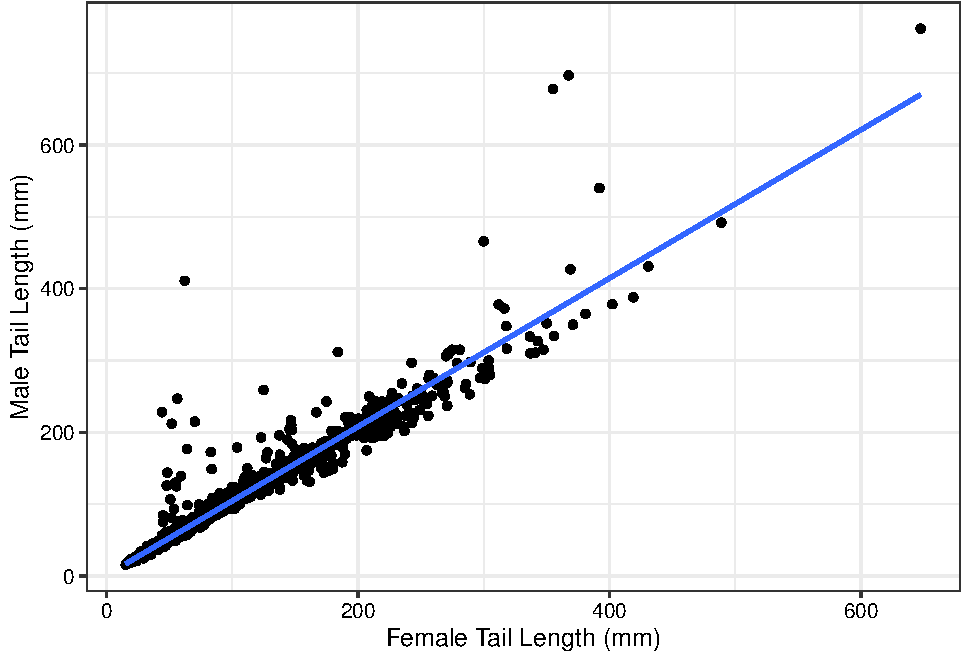
\includegraphics{Project_Code_files/figure-latex/r exploratory_plots_3-1.pdf}
\caption{The Relationship between Female and Male Tail Length}
\end{figure}

\newpage

To visualize the relationship between male and female tail length
another way, here are the distributions of tail length sorted by family
and divided by sex.

\begin{figure}
\centering
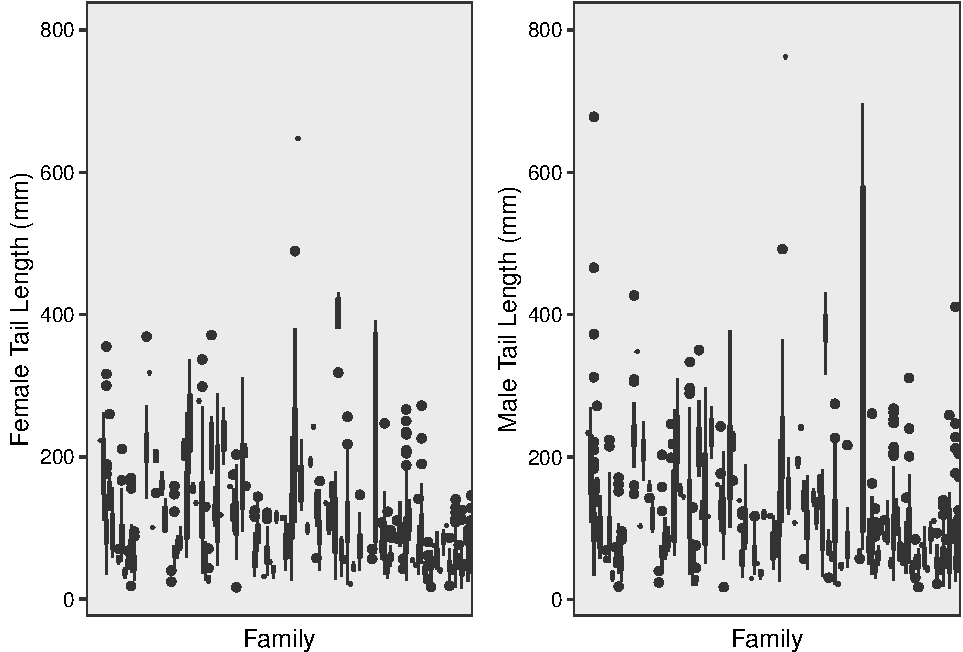
\includegraphics{Project_Code_files/figure-latex/r exploratory_plots_1-1.pdf}
\caption{Exploratory Plots of Tail Length by Sex and Family}
\end{figure}

\hypertarget{exploratory-plots-for-part-2}{%
\subsubsection{Exploratory Plots for Part
2}\label{exploratory-plots-for-part-2}}

In preparation for the second part of our analysis, the following plots
show the distribution of male tail length according to each behavioral
variable: mating system, display system, and resource system.

\begin{figure}
\centering
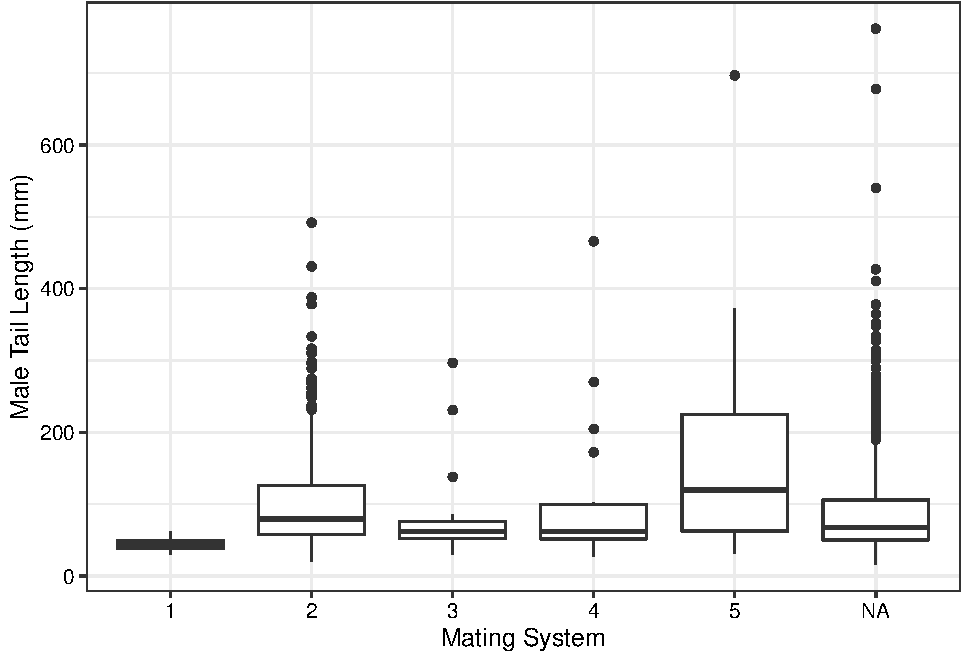
\includegraphics{Project_Code_files/figure-latex/r exploratory_plots_4-1.pdf}
\caption{Male Tail Length by Mating System}
\end{figure}

\begin{figure}
\centering
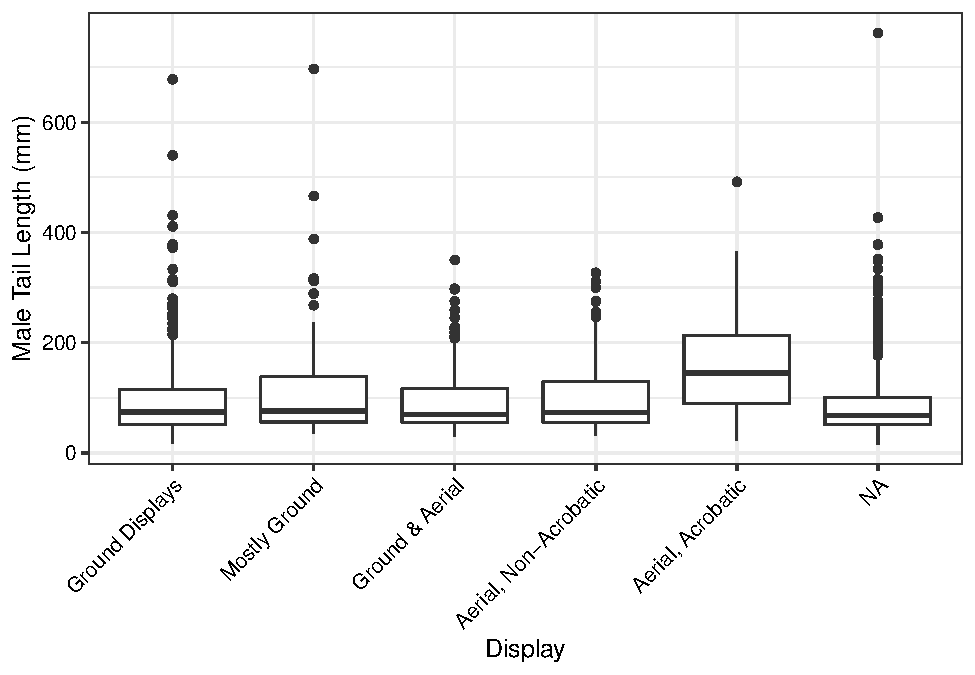
\includegraphics{Project_Code_files/figure-latex/r exploratory_plots_5-1.pdf}
\caption{Male Tail Length by Display System}
\end{figure}

\begin{verbatim}
## Warning: Removed 1379 rows containing non-finite values (stat_boxplot).
\end{verbatim}

\begin{figure}
\centering
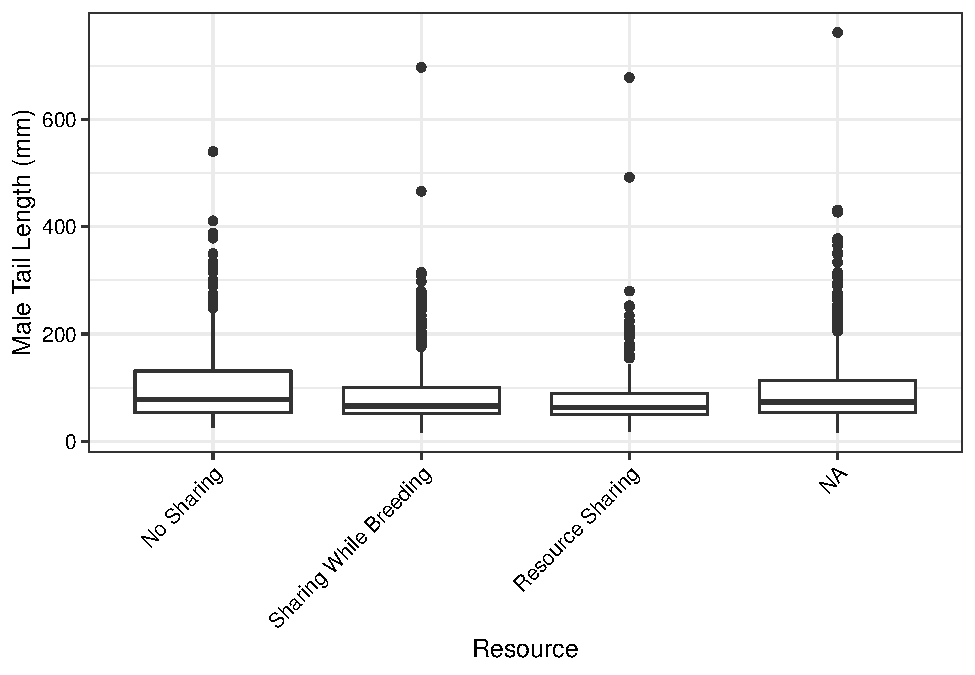
\includegraphics{Project_Code_files/figure-latex/exploratory_plots_6-1.pdf}
\caption{Male Tail Length by Resource System}
\end{figure}

\newpage

\hypertarget{analysis}{%
\section{Analysis}\label{analysis}}

To test our hypotheses using our subset data \texttt{birds.subset}, we
will conduct a linear regression and an analysis of variance (ANOVA).
Our first research question will be answered using a linear regression,
while our second will be addressed with an ANOVA. Results will be stated
in words and supplemented using graphing visualizations.

\hypertarget{question-1-does-female-tail-length-predict-clutch-size}{%
\subsection{Question 1: Does female tail length predict clutch
size?}\label{question-1-does-female-tail-length-predict-clutch-size}}

\(H_0\) : There is no significant difference between female tail length
and clutch size.

\(H_A\) : There is a significant difference between female tail length
and clutch size.

Prior to conducting this analysis, it was identified that there is a
strong correlation between female mass and female tail length. This
makes sense: in general, bigger birds will have longer tails. We
therefore included the mass variable in our model, in order to measure
the effect of tail on clutch size while controlling for the effect of
mass.

\hypertarget{model}{%
\subsubsection{Model}\label{model}}

\begin{verbatim}
## 
## Call:
## lm(formula = Clutch_size ~ F_tail * F_mass)
## 
## Residuals:
##     Min      1Q  Median      3Q     Max 
## -4.9660 -1.2529 -0.2852  0.7347 11.9351 
## 
## Coefficients:
##                    Estimate    Std. Error t value  Pr(>|t|)    
## (Intercept)    3.8970630035  0.0920673618  42.328   < 2e-16 ***
## F_tail        -0.0038295564  0.0009331300  -4.104 0.0000426 ***
## F_mass         0.0002587737  0.0000979394   2.642   0.00832 ** 
## F_tail:F_mass -0.0000010753  0.0000004436  -2.424   0.01546 *  
## ---
## Signif. codes:  0 '***' 0.001 '**' 0.01 '*' 0.05 '.' 0.1 ' ' 1
## 
## Residual standard error: 1.891 on 1642 degrees of freedom
##   (2123 observations deleted due to missingness)
## Multiple R-squared:  0.02398,    Adjusted R-squared:  0.02219 
## F-statistic: 13.45 on 3 and 1642 DF,  p-value: 0.00000001141
\end{verbatim}

Yes, both mass and tail and their interaction are significant (p
\textless{} 0.001). We can reject the null hypothesis and conclude that
mass and tail predict clutch size.

\hypertarget{assumptions}{%
\subsubsection{Assumptions}\label{assumptions}}

Check for multicollinearity. A VIF score below 5 indicates an acceptable
level of multicollinearity:

\begin{verbatim}
##        F_tail        F_mass F_tail:F_mass 
##      1.564475      4.086442      4.876822
\end{verbatim}

\hypertarget{residuals}{%
\subsubsection{Residuals}\label{residuals}}

Next, view residual plots:

\begin{figure}
\centering
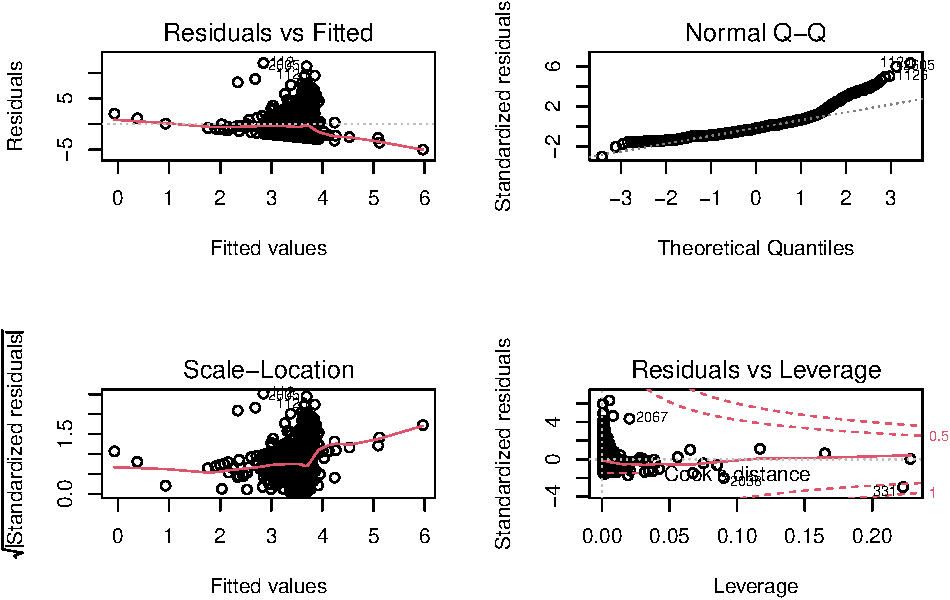
\includegraphics{Project_Code_files/figure-latex/q-1_residuals-1.pdf}
\caption{Residual Plots for Question 1}
\end{figure}

\newpage

\hypertarget{clutch-size-by-tail-length}{%
\subsubsection{Clutch Size by Tail
Length}\label{clutch-size-by-tail-length}}

Below: clutch size declines with increasing female tail length.

\begin{figure}
\centering
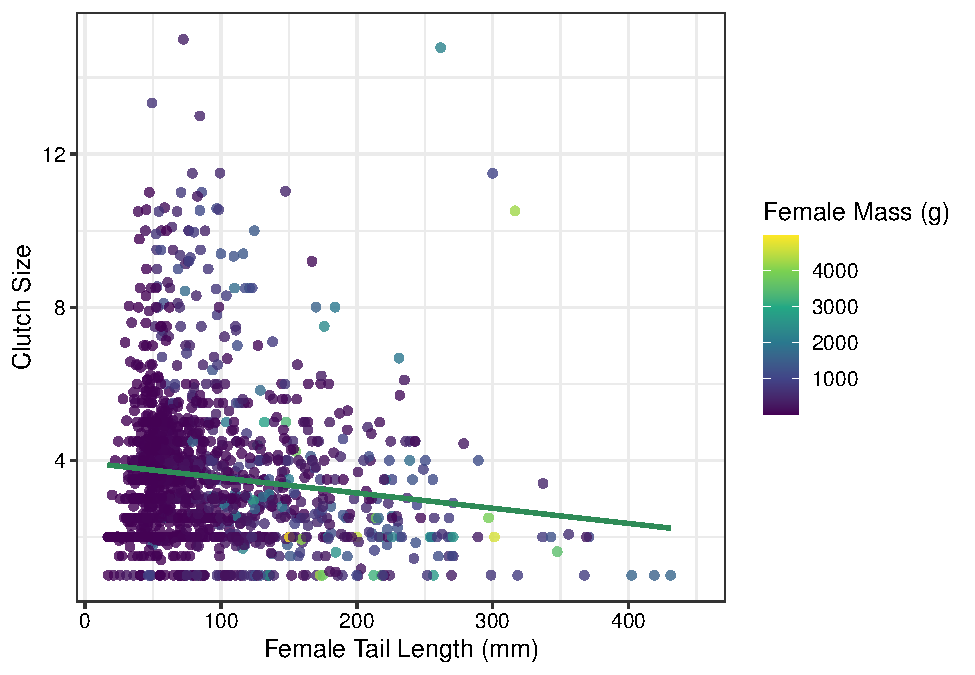
\includegraphics{Project_Code_files/figure-latex/q-1_plot_main-1.pdf}
\caption{Female Tail Length vs Clutch Size}
\end{figure}

\newpage

\hypertarget{question-2-does-male-tail-length-relate-to-mating-approaches}{%
\subsection{Question 2: Does male tail length relate to mating
approaches?}\label{question-2-does-male-tail-length-relate-to-mating-approaches}}

\(H_0\) : Mating system and display behavior do not predict tail size.

\(H_A\) : Mating system and/or display behavior do predict tail size.

\hypertarget{assumptions-1}{%
\subsubsection{Assumptions}\label{assumptions-1}}

First, test for normality and equal variance:

\begin{verbatim}
## 
##  Shapiro-Wilk normality test
## 
## data:  birds.subset$M_tail
## W = 0.75655, p-value < 2.2e-16
\end{verbatim}

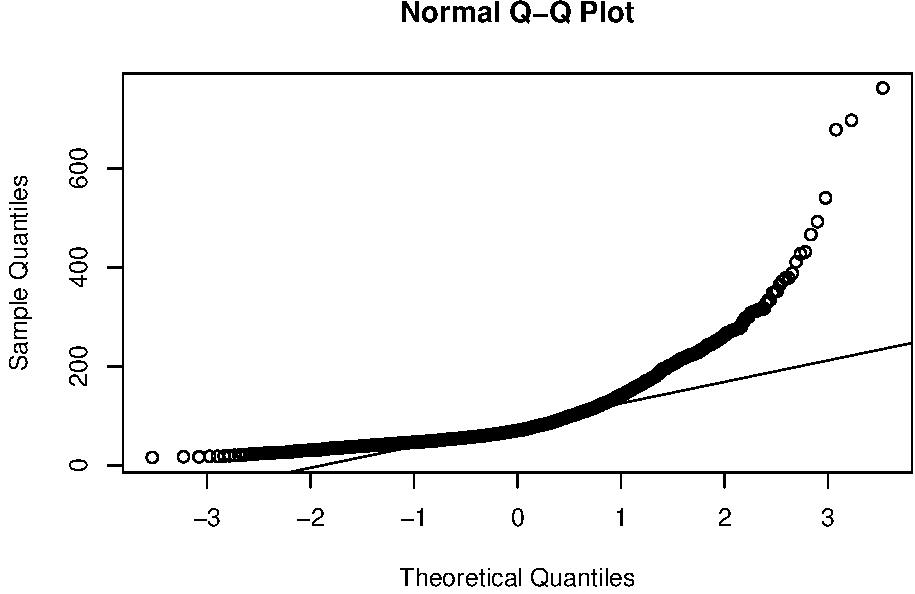
\includegraphics{Project_Code_files/figure-latex/question_2_part_1-1.pdf}

\begin{verbatim}
## 
##  Bartlett test of homogeneity of variances
## 
## data:  M_tail by Mating_System
## Bartlett's K-squared = 102.13, df = 4, p-value < 2.2e-16
\end{verbatim}

\begin{verbatim}
## 
##  Bartlett test of homogeneity of variances
## 
## data:  M_tail by Display
## Bartlett's K-squared = 71.043, df = 4, p-value = 0.00000000000001367
\end{verbatim}

A p-value below the 0.05 threshold from the Bartlett Test indicates that
the variances differ significantly for both Mating System and Display
System.

\hypertarget{model-reduction}{%
\subsubsection{Model Reduction}\label{model-reduction}}

Next, run the model:

\begin{Shaded}
\begin{Highlighting}[]
\NormalTok{mating.anova }\OtherTok{\textless{}{-}} \FunctionTok{aov}\NormalTok{(}\AttributeTok{data =}\NormalTok{ birds.subset, M\_tail }\SpecialCharTok{\textasciitilde{}}\NormalTok{ Mating\_System }\SpecialCharTok{*}\NormalTok{ Display }\SpecialCharTok{*}\NormalTok{ Resource)}
\FunctionTok{summary}\NormalTok{(mating.anova)}
\end{Highlighting}
\end{Shaded}

\begin{verbatim}
##                                 Df  Sum Sq Mean Sq F value            Pr(>F)
## Mating_System                    4   59317   14829   3.548           0.00737
## Display                          4  164931   41233   9.865 0.000000129331941
## Resource                         2   18622    9311   2.228           0.10914
## Mating_System:Display           11  377637   34331   8.214 0.000000000000544
## Mating_System:Resource           3   13812    4604   1.102           0.34832
## Display:Resource                 8   35663    4458   1.067           0.38570
## Mating_System:Display:Resource   4   12473    3118   0.746           0.56109
## Residuals                      393 1642577    4180                          
##                                   
## Mating_System                  ** 
## Display                        ***
## Resource                          
## Mating_System:Display          ***
## Mating_System:Resource            
## Display:Resource                  
## Mating_System:Display:Resource    
## Residuals                         
## ---
## Signif. codes:  0 '***' 0.001 '**' 0.01 '*' 0.05 '.' 0.1 ' ' 1
## 3339 observations deleted due to missingness
\end{verbatim}

Because not everything was significant, we used a nested model approach
to reduce the model until all components were significant.

\newpage

Here is the final model:

\begin{Shaded}
\begin{Highlighting}[]
\NormalTok{mating.anova.final }\OtherTok{\textless{}{-}} \FunctionTok{aov}\NormalTok{(}\AttributeTok{data =}\NormalTok{ birds.subset, M\_tail }\SpecialCharTok{\textasciitilde{}}\NormalTok{ Mating\_System }\SpecialCharTok{*}\NormalTok{ Display)}
\FunctionTok{summary}\NormalTok{(mating.anova.final)}
\end{Highlighting}
\end{Shaded}

\begin{verbatim}
##                        Df  Sum Sq Mean Sq F value     Pr(>F)    
## Mating_System           4  135625   33906   7.198 0.00001259 ***
## Display                 4  148286   37071   7.870 0.00000386 ***
## Mating_System:Display  12  229022   19085   4.052 0.00000526 ***
## Residuals             455 2143223    4710                       
## ---
## Signif. codes:  0 '***' 0.001 '**' 0.01 '*' 0.05 '.' 0.1 ' ' 1
## 3293 observations deleted due to missingness
\end{verbatim}

The interaction between mating system and display system is significant
(p \textless{} 0.001). We can reject the null hypothesis and accept that
mating system and display system predict male tail length.

\hypertarget{residuals-1}{%
\subsubsection{Residuals}\label{residuals-1}}

\begin{figure}
\centering
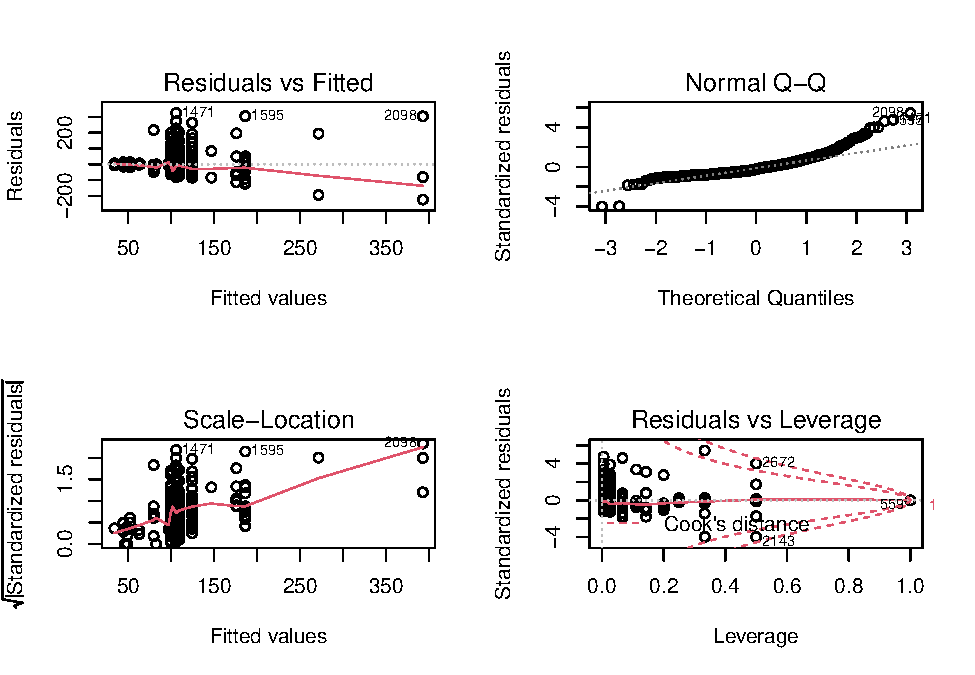
\includegraphics{Project_Code_files/figure-latex/q-2 residual-1.pdf}
\caption{Residual Plots for Question 2}
\end{figure}

\newpage

\hypertarget{tail-length-by-mating-and-display-systems}{%
\subsubsection{Tail Length by Mating and Display
Systems}\label{tail-length-by-mating-and-display-systems}}

Below, average male tail length by mating system and display system.

\begin{figure}
\centering
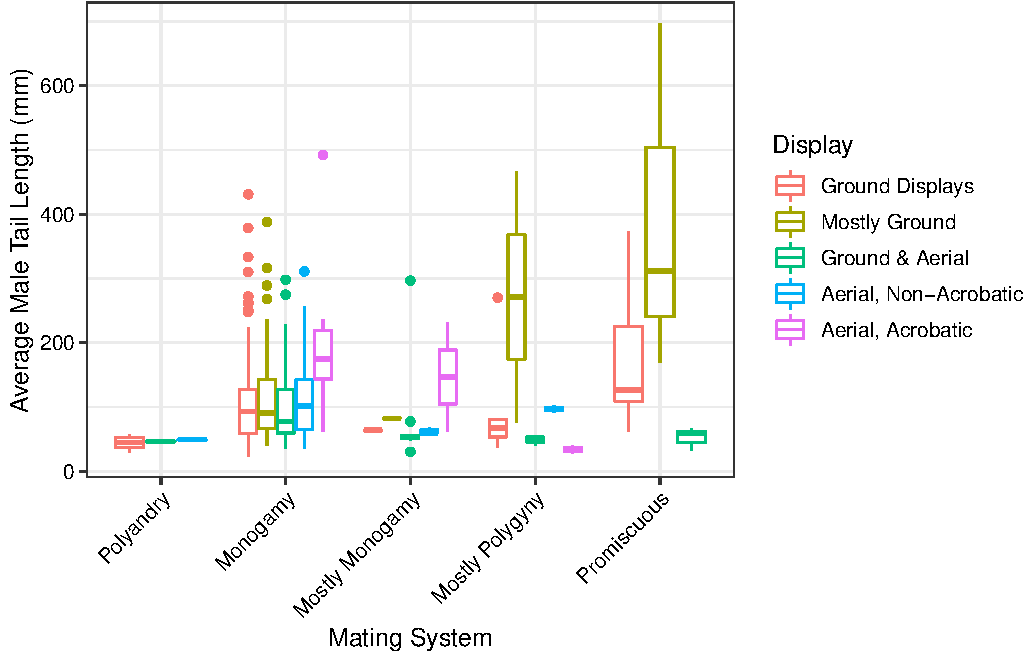
\includegraphics{Project_Code_files/figure-latex/q-2-plots-1.pdf}
\caption{Male Tail Length vs Mating Tactics}
\end{figure}

\newpage

Below, the same results as the previous page but with the mating system
and display system swapped.
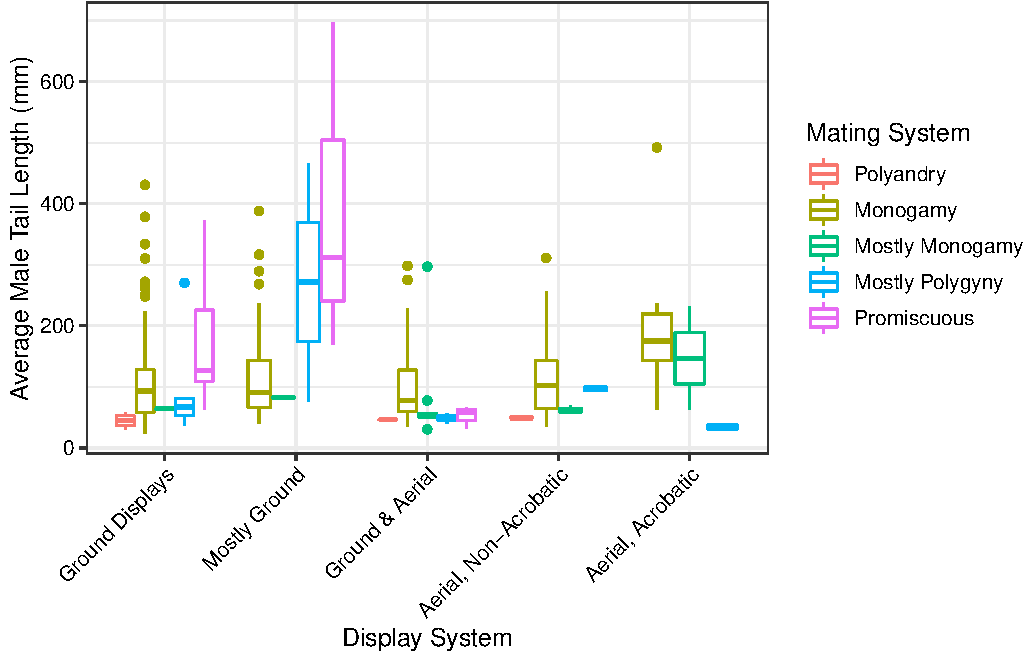
\includegraphics{Project_Code_files/figure-latex/q-2-plots2-1.pdf}

\newpage

\hypertarget{summary-and-conclusions}{%
\section{Summary and Conclusions}\label{summary-and-conclusions}}

\hypertarget{part-1}{%
\subsection{Part 1}\label{part-1}}

The interaction between female mass and tail size predicts clutch size
(p \textless{} 0.001, n = 1642, R\textsuperscript{2} = 0.022). In
general, clutch size appears to decrease with increasing tail length,
but this effect is mediated by overall body size as expressed by mass.

However, it is important to note the limitations of our model. Our model
does not explain much of the variance, as seen from our low
R\textsuperscript{2} value. We can also see that the residual plots are
quite clumped together in each plot at a different location. More
explanatory variables should be used to determine the impact of female
mass and tail size on clutch size.

Our finding supports the hypothesis that birds with longer tails may
expend more resources collecting food because of their reduced agility.
Therefore, they may have adapted to produce fewer eggs because they
cannot care for as many chicks as more agile birds. More research is
needed to substantiate this hypothesis as well as to better understand
how overall body size mediates the effect.

\begin{figure}
\centering
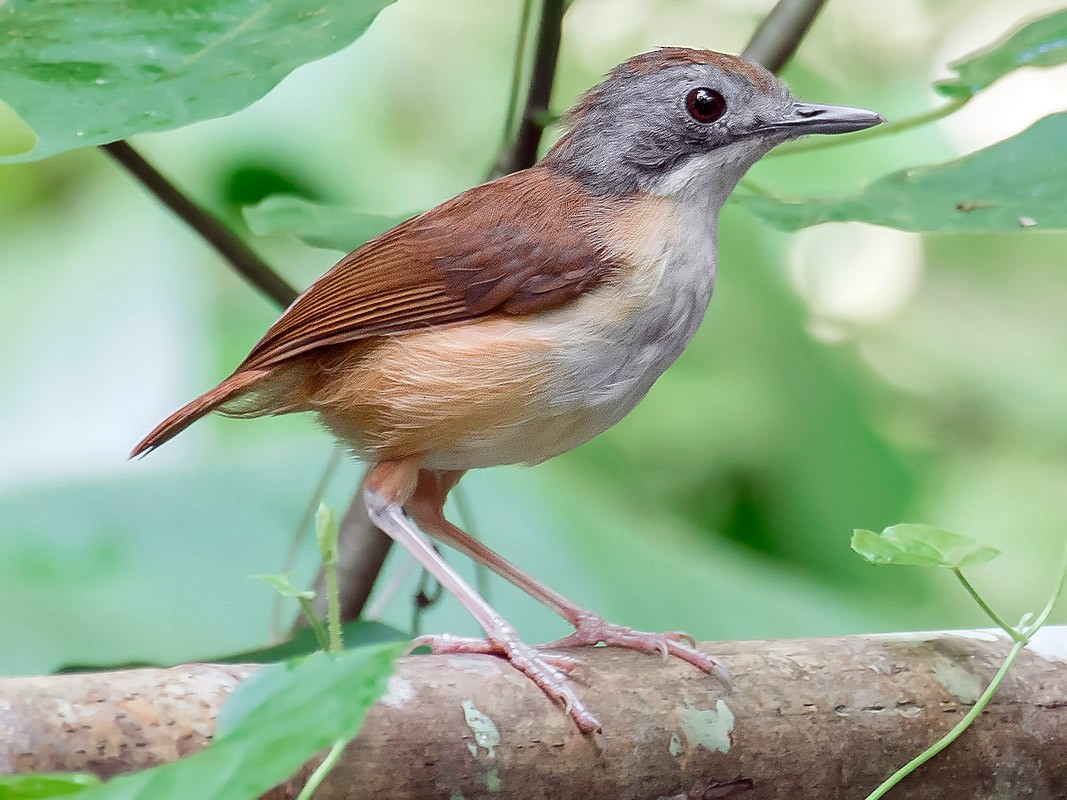
\includegraphics{Images/short-tailed_babbler.jpeg}
\caption{A Short-tailed Babbler (\emph{Pellorneum malaccense})}
\end{figure}

\newpage

\hypertarget{part-2}{%
\subsection{Part 2}\label{part-2}}

Mating system and display system interact to predict tail length (n =
476, p \textless{} 0.001), supporting our hypothesis. In general, mostly
polygynous and promiscuous birds with mostly ground displays appear to
have the longest tails. Among monogamous and mostly monogamous birds,
those with aerial displays have the longest tails.

This said, it should be noted that tail length is not normally
distributed, and could be transformed in future analysis to meet the
normality assumption. Groups in this analysis also do not have equal
variance. For example, in Mating System, most birds are identified as
monogamous (2), leading to a skew in the data, not because of lack of
samples but rather lack of diversity in this category. Similarly to part
one, we find clumps of data points in the residual plots, but in this
case they seem to reflect the unequal grouping of variables used within
this analysis. There are vertical groups that are distinguishable across
all plots, which is something that should be explored in the future, as
an attempt to correct this or eliminate its overall impact on the data.

Our result indicates that birds vary in tail length according to both
their mating system and their display system. This finding is not
surprising considering that male birds with particularly long tails are
known to use them in courtship displays, so species of birds have
developed varied tail lengths alongside specific mating behaviors. We
chose not to control for overall mass in this model because increasingly
complex statistical analyses are outside of the scope covered in this
course, but the lack of control is a definitive limitation of this
finding: some patterns of mating system and display predicting tail
length may be a result of overall size rather than tail length
specifically. More research and analyses are needed.

\begin{figure}
\centering
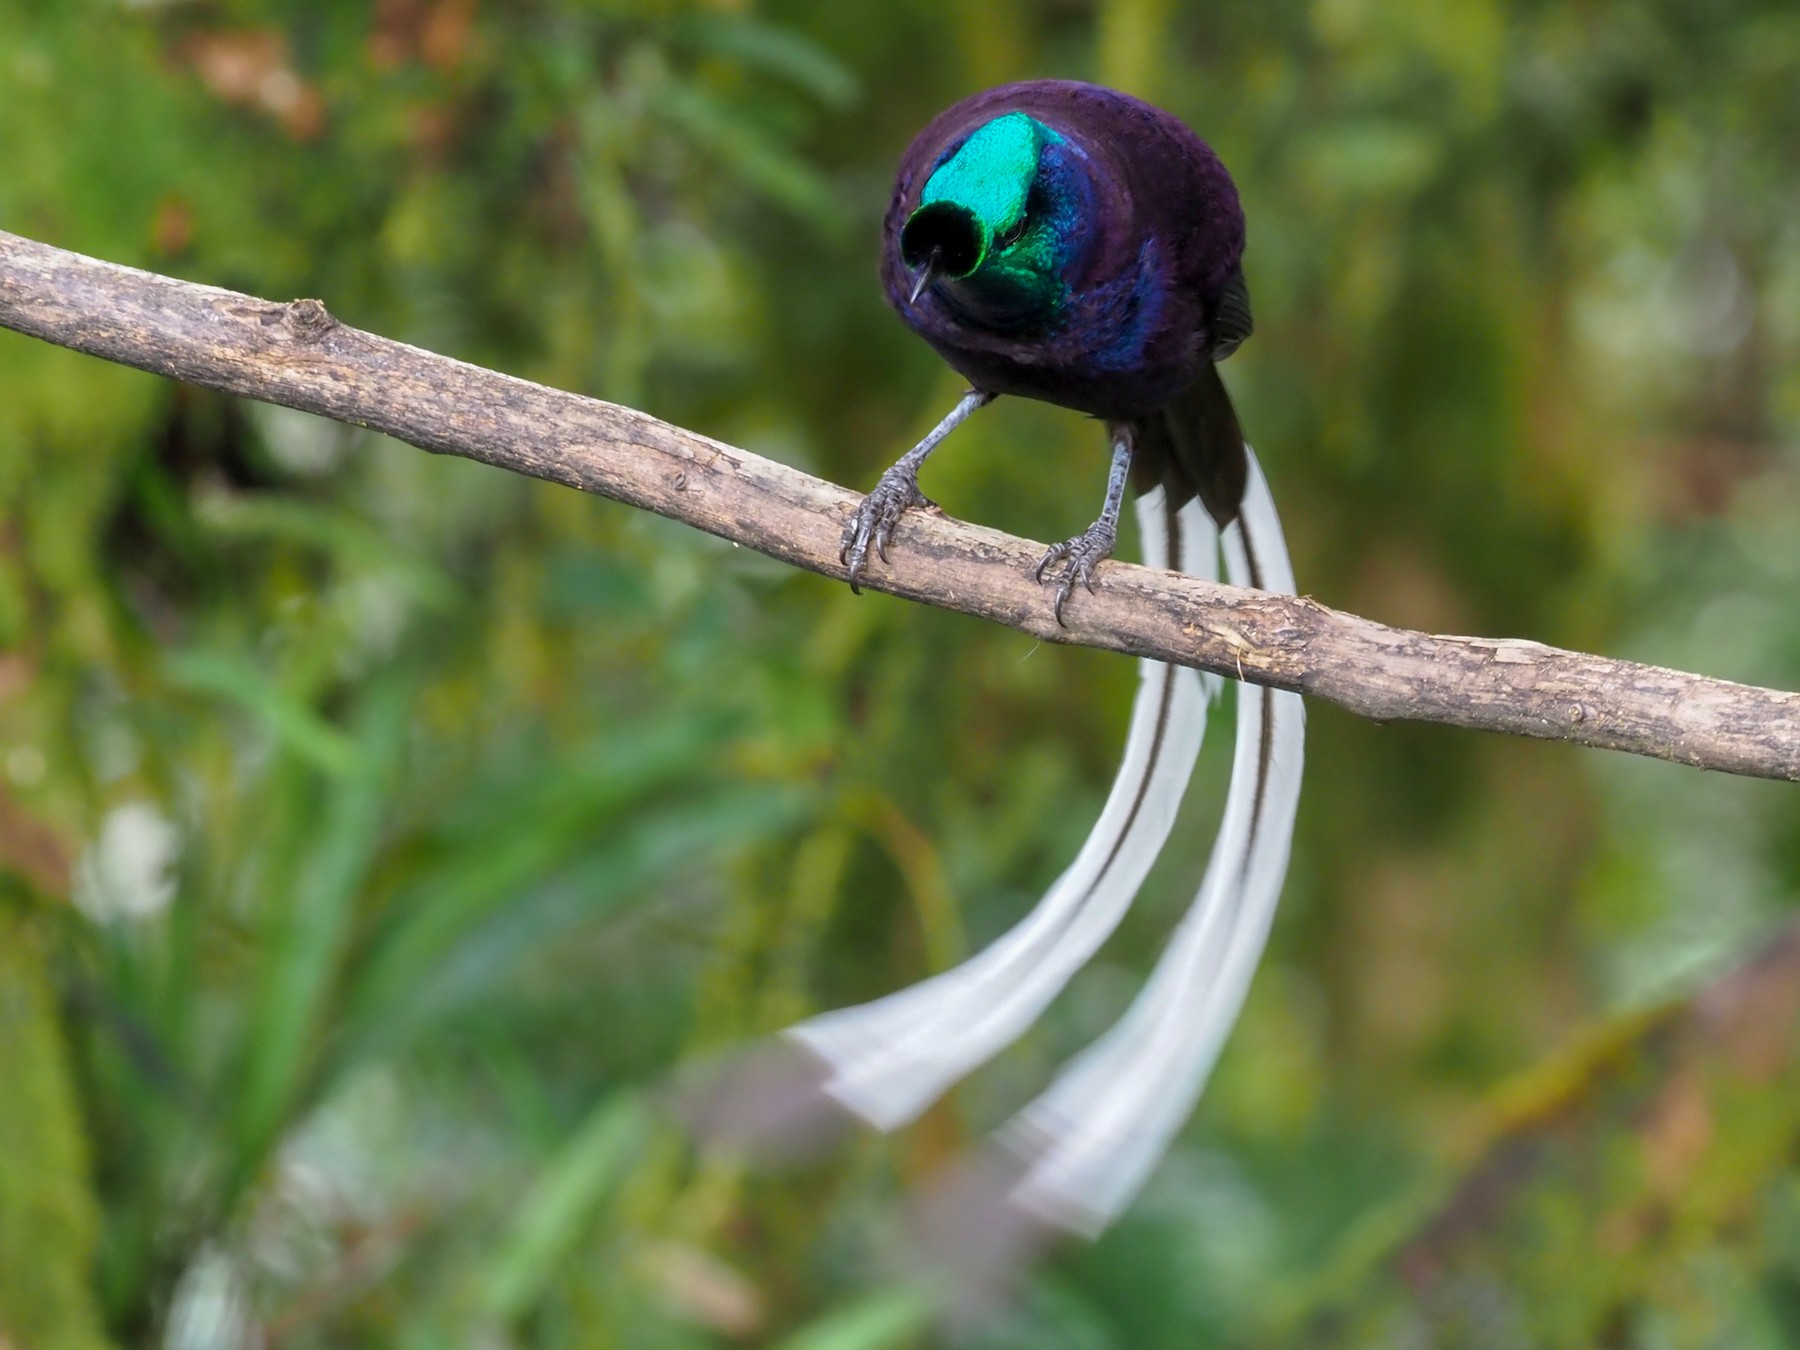
\includegraphics{Images/ribbon-tailed_astrapia.jpeg}
\caption{A Male Ribbon-tailed Astrapia (\emph{Astrapia mayeri})}
\end{figure}

\newpage

\hypertarget{references}{%
\section{References}\label{references}}

\begin{itemize}
\item
  Chotjuckdikul, N. 2017. Short-tailed Babbler: \emph{Pellorneum
  malaccense.} eBird. \url{https://ebird.org/species/shtbab1}
\item
  Evans, M.R. 1999. The consequences of flight for the evolution of tail
  ornaments in birds. In: Adams, N.J. \& Slotow, R.H. (eds) \emph{Proc.
  22 Int. Ornithol. Congr.,} Durban: 1823-1843. Johannesburg: BirdLife
  South Africa.
\item
  Jearwattanakanok, A. 2019. Great Argus: \emph{Argusianus argus.}
  eBird. \url{https://ebird.org/species/grearg1}
\item
  Lislevand, T., Figuerola, J., and Székely, T. 2007. Avian body sizes
  in relation to fecundity, mating system, display behavior, and
  resource sharing. \emph{Ecology} 88:1605.
\item
  Lorenz, S. 2019. Ribbon-tailed Astrapia: \emph{Astrapia mayeri.}
  eBird. \url{https://ebird.org/species/ritast1}
\end{itemize}

\end{document}
